% ==============================================================
% WORKFLOW DIAGRAMS — All three detailed flowcharts (TikZ)
% NOTE: node names must NOT contain underscores (TikZ csname issue)
% ==============================================================
\usetikzlibrary{shapes.geometric,arrows.meta,positioning,fit,backgrounds,calc}

% ==============================================================
% FIGURE 1 — Entry routing: Firmware + AI Discovery + Web exit
% ==============================================================
\begin{figure}[htbp]
\centering
\resizebox{\textwidth}{!}{%
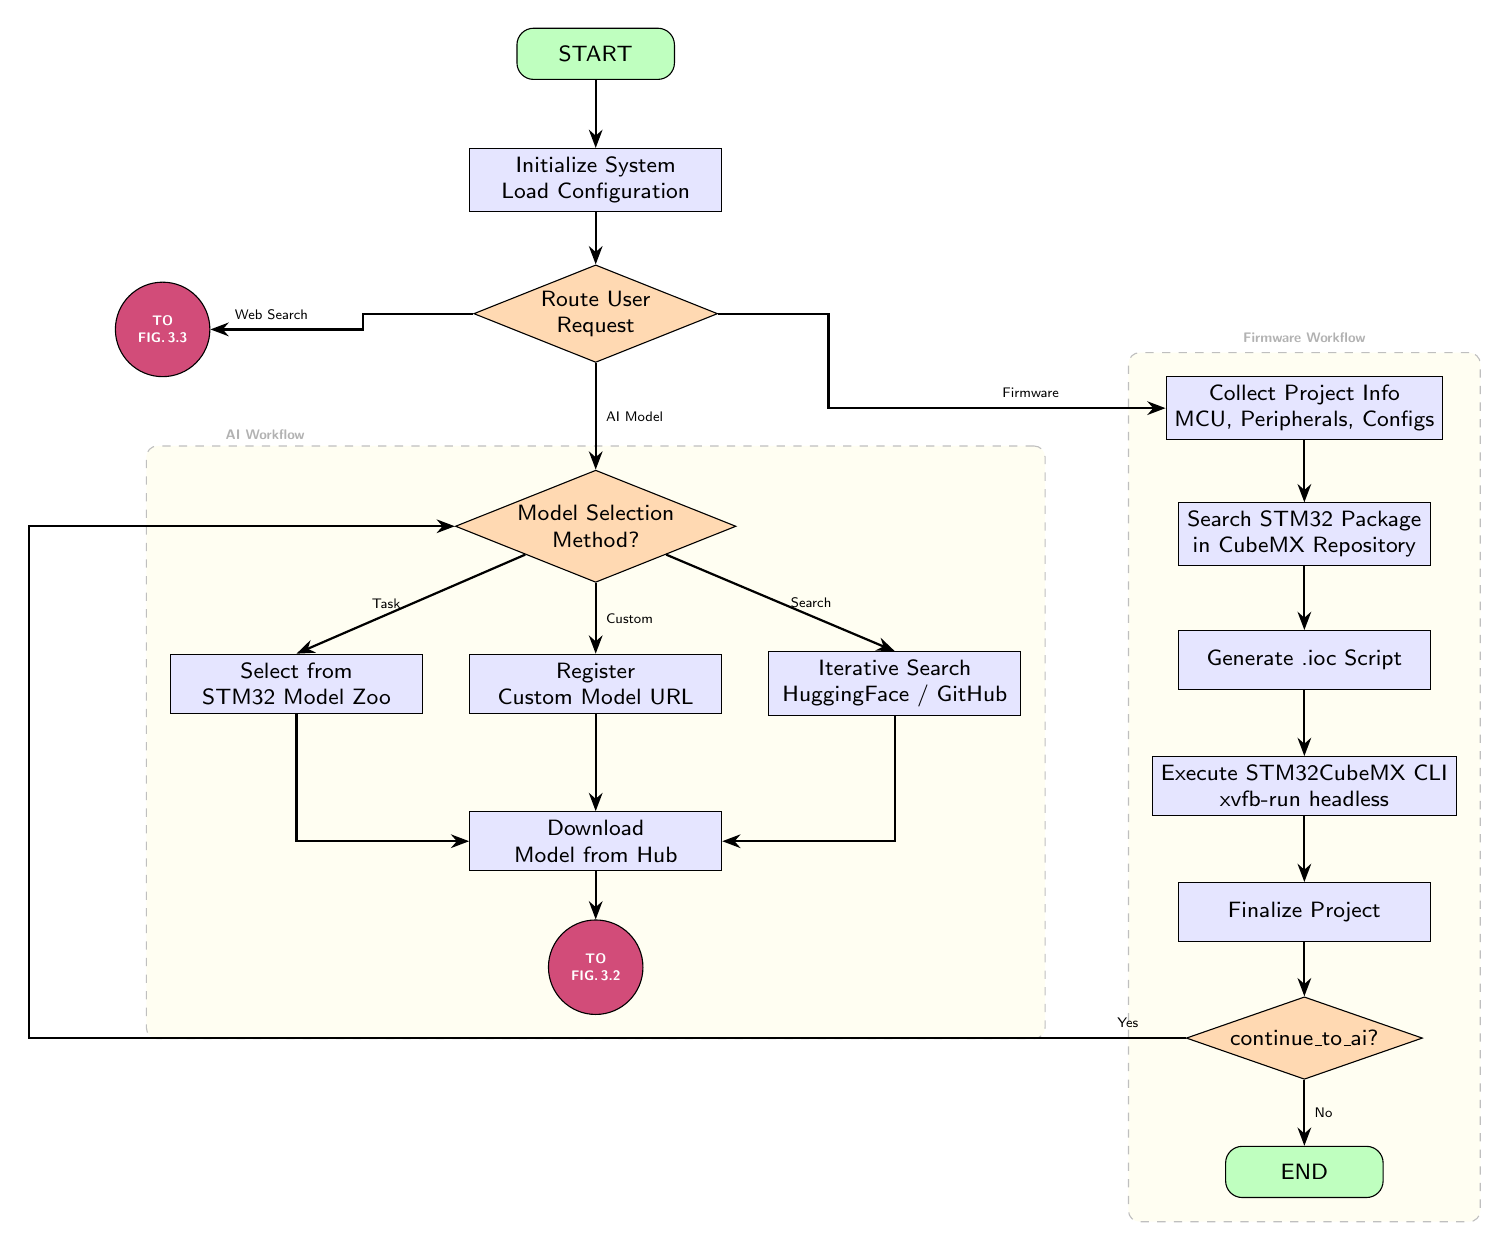
\begin{tikzpicture}[
  every node/.style={font=\sffamily\footnotesize},
  proc/.style={draw, fill=blue!10, rectangle, minimum width=3.2cm,
               minimum height=0.75cm, align=center, inner sep=3pt},
  dec/.style={draw, fill=orange!30, diamond, aspect=2.5,
              align=center, inner sep=1pt, minimum width=3cm, minimum height=1cm},
  se/.style={draw, rectangle, rounded corners=6pt, fill=green!25,
             minimum width=2cm, minimum height=0.65cm, align=center},
  co/.style={draw, circle, fill=purple!70, text=white, minimum size=1.2cm,
             align=center, font=\sffamily\tiny\bfseries},
  wb/.style={draw=gray!50, dashed, rounded corners=4pt, fill=yellow!5, inner sep=0.3cm},
  ar/.style={->, thick, >=Stealth}]

%% --- Shared top ---
\node[se]   (START)  at (0,     0)    {START};
\node[proc] (INIT)   at (0,    -1.6)  {Initialize System \\ Load Configuration};
\node[dec]  (ROUTE)  at (0,    -3.3)  {Route User \\ Request};

%% --- Web exit (left) ---
\node[co]   (WSOUT)  at (-5.5, -3.5)  {TO \\ FIG.\,3.3};

%% --- AI Discovery (centre) — shifted down for label readability ---
\node[dec]  (AISEL)  at ( 0.0, -6.0)  {Model Selection \\ Method?};
\node[proc] (AITASK) at (-3.8, -8.0)  {Select from \\ STM32 Model Zoo};
\node[proc] (AIURL)  at ( 0.0, -8.0)  {Register \\ Custom Model URL};
\node[proc] (AIWS)   at ( 3.8, -8.0)  {Iterative Search \\ HuggingFace / GitHub};
\node[proc] (AIDL)   at ( 0.0,-10.0)  {Download \\ Model from Hub};
\node[co]   (OUTAI)  at ( 0.0,-11.6)  {TO \\ FIG.\,3.2};

%% --- Firmware (right) ---
\node[proc] (FWA)    at (9.0, -4.5)  {Collect Project Info \\ MCU, Peripherals, Configs};
\node[proc] (FWB)    at (9.0, -6.1)  {Search STM32 Package \\ in CubeMX Repository};
\node[proc] (FWC)    at (9.0, -7.7)  {Generate .ioc Script};
\node[proc] (FWD)    at (9.0, -9.3)  {Execute STM32CubeMX CLI \\ xvfb-run headless};
\node[proc] (FWE)    at (9.0,-10.9)  {Finalize Project};
\node[dec]  (FWCONT) at (9.0,-12.5)  {continue\_to\_ai?};
\node[se]   (ENDA)   at (9.0,-14.2)  {END};

%% --- Arrows: top ---
\draw[ar] (START) -- (INIT);
\draw[ar] (INIT)  -- (ROUTE);
\draw[ar] (ROUTE.west)  -- ++(-1.4,0) |- node[above,pos=0.8,font=\sffamily\tiny]{Web Search} (WSOUT);
\draw[ar] (ROUTE.south) -- node[right,font=\sffamily\tiny]{AI Model} (AISEL.north);
\draw[ar] (ROUTE.east)  -- ++(1.4,0)  |- node[above,pos=0.8,font=\sffamily\tiny]{Firmware}   (FWA.west);

%% --- Arrows: AI Discovery ---
\draw[ar] (AISEL.south west) -- node[left, font=\sffamily\tiny]{Task}   (AITASK.north);
\draw[ar] (AISEL.south)      -- node[right,font=\sffamily\tiny]{Custom} (AIURL.north);
\draw[ar] (AISEL.south east) -- node[right,font=\sffamily\tiny]{Search} (AIWS.north);
\draw[ar] (AITASK.south) |- (AIDL.west);
\draw[ar] (AIURL.south)  --  (AIDL.north);
\draw[ar] (AIWS.south)   |- (AIDL.east);
\draw[ar] (AIDL) -- (OUTAI);

%% --- Arrows: Firmware ---
\draw[ar] (FWA) -- (FWB);  \draw[ar] (FWB) -- (FWC);
\draw[ar] (FWC) -- (FWD);  \draw[ar] (FWD) -- (FWE);
\draw[ar] (FWE) -- (FWCONT);
%% YES: loop back left → up → into AISEL (routed outside all blocks at x=-7)
\draw[ar] (FWCONT.west)
    -- node[above,pos=0.05,font=\sffamily\tiny]{Yes}
    (-7.2,-12.5) -- (-7.2,-6.0) -- (AISEL.west);
%% NO: straight down to END
\draw[ar] (FWCONT.south) -- node[right,font=\sffamily\tiny]{No} (ENDA.north);

%% --- Bounding boxes ---
\begin{scope}[on background layer]
  \node[wb, fit=(AISEL)(AITASK)(AIURL)(AIWS)(AIDL)(OUTAI),
        label={[font=\sffamily\tiny\bfseries,text=gray!60,yshift=-0.5mm,xshift=2mm]above left:AI Workflow}]{};
  \node[wb, fit=(FWA)(FWB)(FWC)(FWD)(FWE)(FWCONT)(ENDA),
        label={[font=\sffamily\tiny\bfseries,text=gray!60]above:Firmware Workflow}]{};
\end{scope}
\end{tikzpicture}}
\caption{Detailed Workflow Diagram - System initialization, request routing, and entry workflows (Firmware Generation and AI Model Discovery). Web Search requests exit directly to Figure~\ref{fig:detailed_flowchart_part3}.}
\label{fig:detailed_flowchart_part1}
\end{figure}

% ==============================================================
% FIGURE 2 — Model Customization (Workflow 5), snake layout
% ==============================================================
\begin{figure}[htbp]
\centering
\resizebox{\textwidth}{!}{%
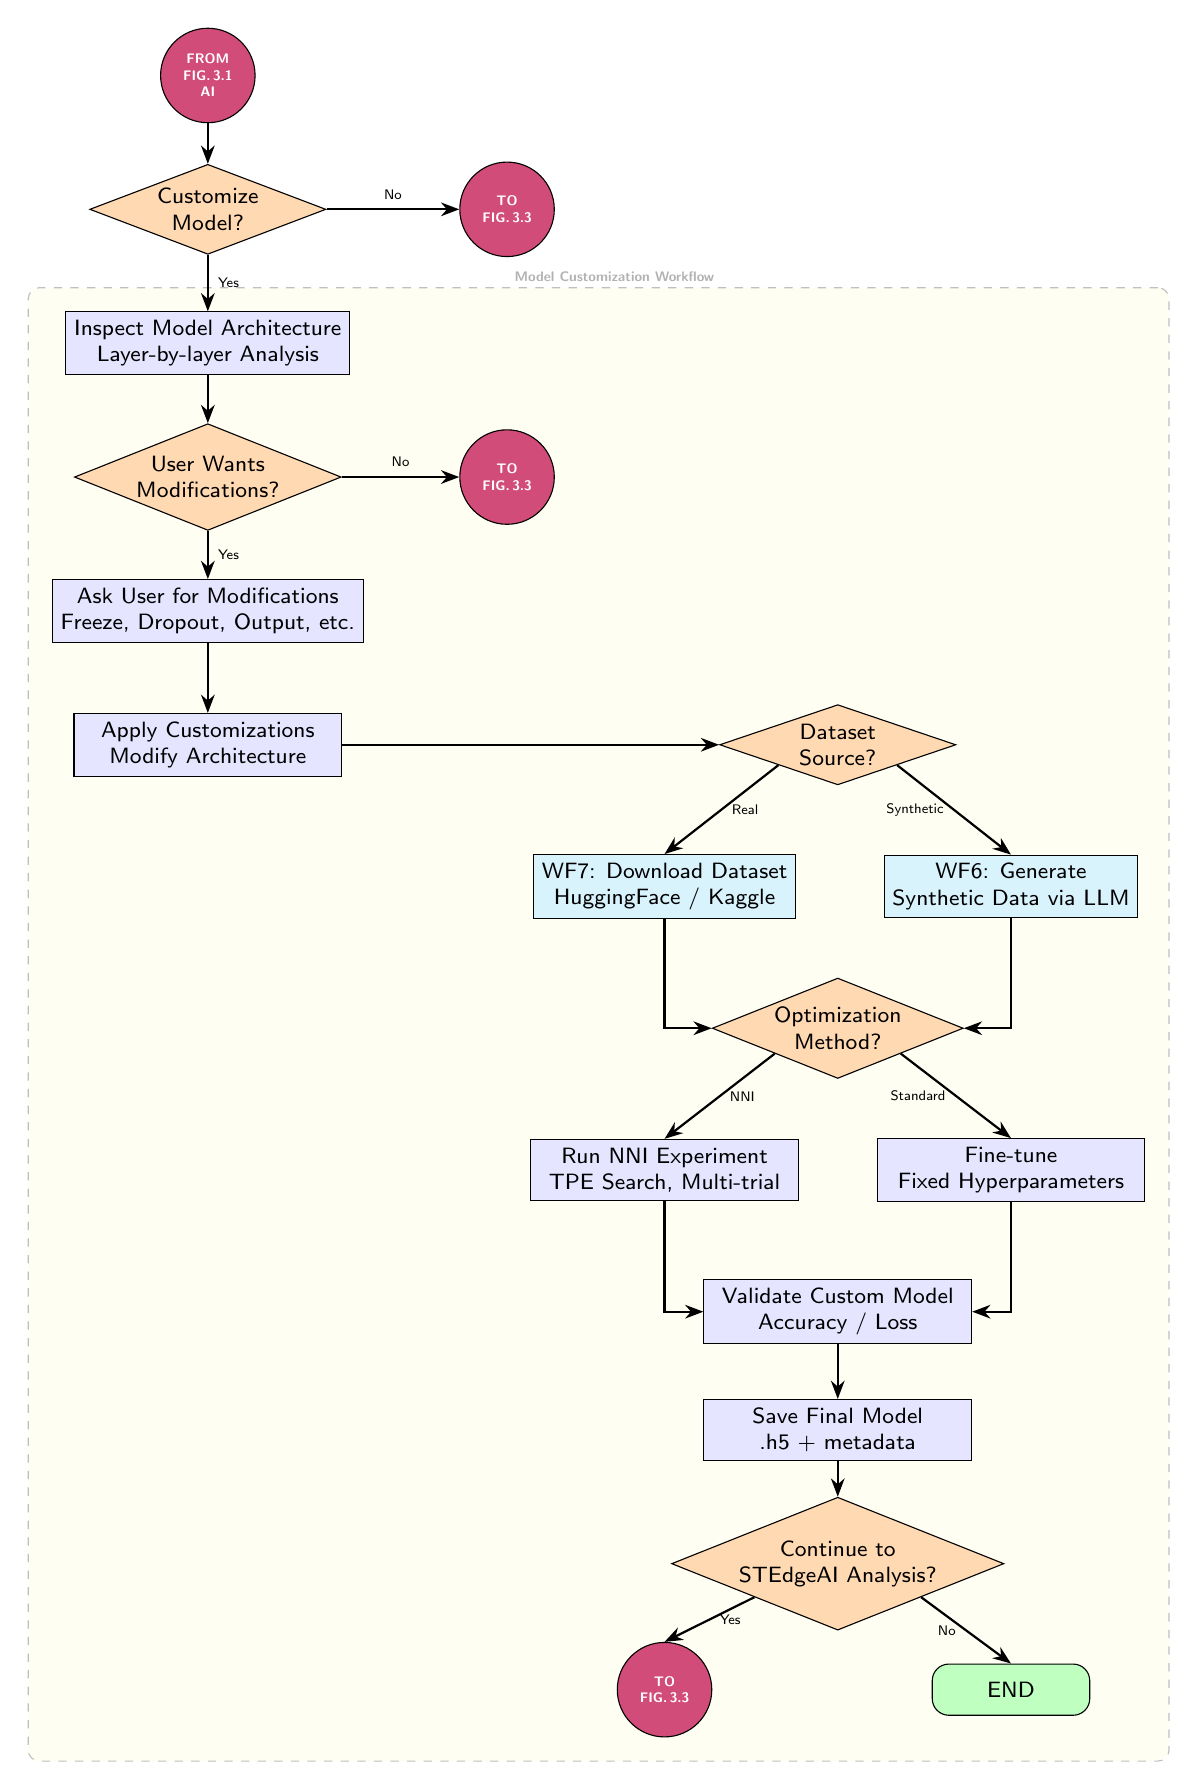
\begin{tikzpicture}[
  every node/.style={font=\sffamily\footnotesize},
  proc/.style={draw, fill=blue!10, rectangle, minimum width=3.4cm,
               minimum height=0.75cm, align=center, inner sep=3pt},
  psub/.style={draw, fill=cyan!15, rectangle, minimum width=3.0cm,
               minimum height=0.75cm, align=center, inner sep=3pt},
  dec/.style={draw, fill=orange!30, diamond, aspect=2.5,
              align=center, inner sep=1pt, minimum width=3cm, minimum height=1cm},
  se/.style={draw, rectangle, rounded corners=6pt, fill=green!25,
             minimum width=2cm, minimum height=0.65cm, align=center},
  co/.style={draw, circle, fill=purple!70, text=white, minimum size=1.2cm,
             align=center, font=\sffamily\tiny\bfseries},
  wb/.style={draw=gray!50, dashed, rounded corners=4pt, fill=yellow!5, inner sep=0.3cm},
  ar/.style={->, thick, >=Stealth}]

%% ---- COLUMN 1 (x=0, top-down) ----
\node[co]   (FRA)  at ( 0,    0)   {FROM \\ FIG.\,3.1 \\ AI};
\node[dec]  (CUST) at ( 0,  -1.7) {Customize \\ Model?};
\node[co]   (SKA)  at ( 3.8,-1.7) {TO \\ FIG.\,3.3};
\node[proc] (CUA)  at ( 0,  -3.4) {Inspect Model Architecture \\ Layer-by-layer Analysis};
\node[dec]  (CINT) at ( 0,  -5.1) {User Wants \\ Modifications?};
\node[co]   (SKB)  at ( 3.8,-5.1) {TO \\ FIG.\,3.3};
\node[proc] (CUB)  at ( 0,  -6.8) {Ask User for Modifications \\ Freeze, Dropout, Output, etc.};
\node[proc] (CUC)  at ( 0,  -8.5) {Apply Customizations \\ Modify Architecture};

%% ---- COLUMN 2 (x=8, snake turn) ----
\node[dec]  (CDS)  at (8.0, -8.5)  {Dataset \\ Source?};
\node[psub] (DREA) at (5.8,-10.3)  {WF7: Download Dataset \\ HuggingFace / Kaggle};
\node[psub] (DSYN) at (10.2,-10.3) {WF6: Generate \\ Synthetic Data via LLM};
\node[dec]  (COPT) at (8.0,-12.1)  {Optimization \\ Method?};
\node[proc] (CNNI) at (5.8,-13.9)  {Run NNI Experiment \\ TPE Search, Multi-trial};
\node[proc] (CSTD) at (10.2,-13.9) {Fine-tune \\ Fixed Hyperparameters};
\node[proc] (CVAL) at (8.0,-15.7)  {Validate Custom Model \\ Accuracy / Loss};
\node[proc] (CSAV) at (8.0,-17.2)  {Save Final Model \\ .h5 + metadata};
\node[dec]  (CCON) at (8.0,-18.9)  {Continue to \\ STEdgeAI Analysis?};
\node[co]   (OUY)  at (5.8,-20.5)  {TO \\ FIG.\,3.3};
\node[se]   (ENDB) at (10.2,-20.5) {END};

%% --- Arrows col 1 ---
\draw[ar] (FRA) -- (CUST);
\draw[ar] (CUST.east)  -- node[above,font=\sffamily\tiny]{No}  (SKA.west);
\draw[ar] (CUST.south) -- node[right,font=\sffamily\tiny]{Yes} (CUA.north);
\draw[ar] (CUA)  -- (CINT);
\draw[ar] (CINT.east)  -- node[above,font=\sffamily\tiny]{No}  (SKB.west);
\draw[ar] (CINT.south) -- node[right,font=\sffamily\tiny]{Yes} (CUB.north);
\draw[ar] (CUB) -- (CUC);

%% Snake turn
\draw[ar] (CUC.east) -- (CDS.west);

%% --- Arrows col 2 ---
\draw[ar] (CDS.south west) -- node[right,font=\sffamily\tiny]{Real}      (DREA.north);
\draw[ar] (CDS.south east) -- node[left, font=\sffamily\tiny]{Synthetic} (DSYN.north);
\draw[ar] (DREA.south) |- (COPT.west);
\draw[ar] (DSYN.south) |- (COPT.east);
\draw[ar] (COPT.south west) -- node[right,font=\sffamily\tiny]{NNI}      (CNNI.north);
\draw[ar] (COPT.south east) -- node[left, font=\sffamily\tiny]{Standard} (CSTD.north);
\draw[ar] (CNNI.south) |- (CVAL.west);
\draw[ar] (CSTD.south) |- (CVAL.east);
\draw[ar] (CVAL) -- (CSAV);
\draw[ar] (CSAV) -- (CCON);
\draw[ar] (CCON.south west) -- node[right,font=\sffamily\tiny]{Yes} (OUY.north);
\draw[ar] (CCON.south east) -- node[left, font=\sffamily\tiny]{No}  (ENDB.north);

%% --- Bounding box ---
\begin{scope}[on background layer]
  \node[wb, fit=(CUA)(CINT)(CUB)(CUC)(CDS)(DREA)(DSYN)(COPT)(CNNI)(CSTD)(CVAL)(CSAV)(CCON)(OUY)(ENDB),
        label={[font=\sffamily\tiny\bfseries,text=gray!60, yshift=-0.5mm,xshift=+2mm]above:Model Customization Workflow}]{};
\end{scope}
\end{tikzpicture}}
\caption{Detailed Workflow Diagram - Model customization workflow (Workflow~5). Left column: architecture inspection and modification. Right column: dataset acquisition, hyperparameter optimization via NNI, and model validation.}
\label{fig:detailed_flowchart_part2}
\end{figure}

% ==============================================================
% FIGURE 3 — STEdgeAI + Integration + Web Search
% ==============================================================
\begin{figure}[htbp]
\centering
\resizebox{\textwidth}{!}{%
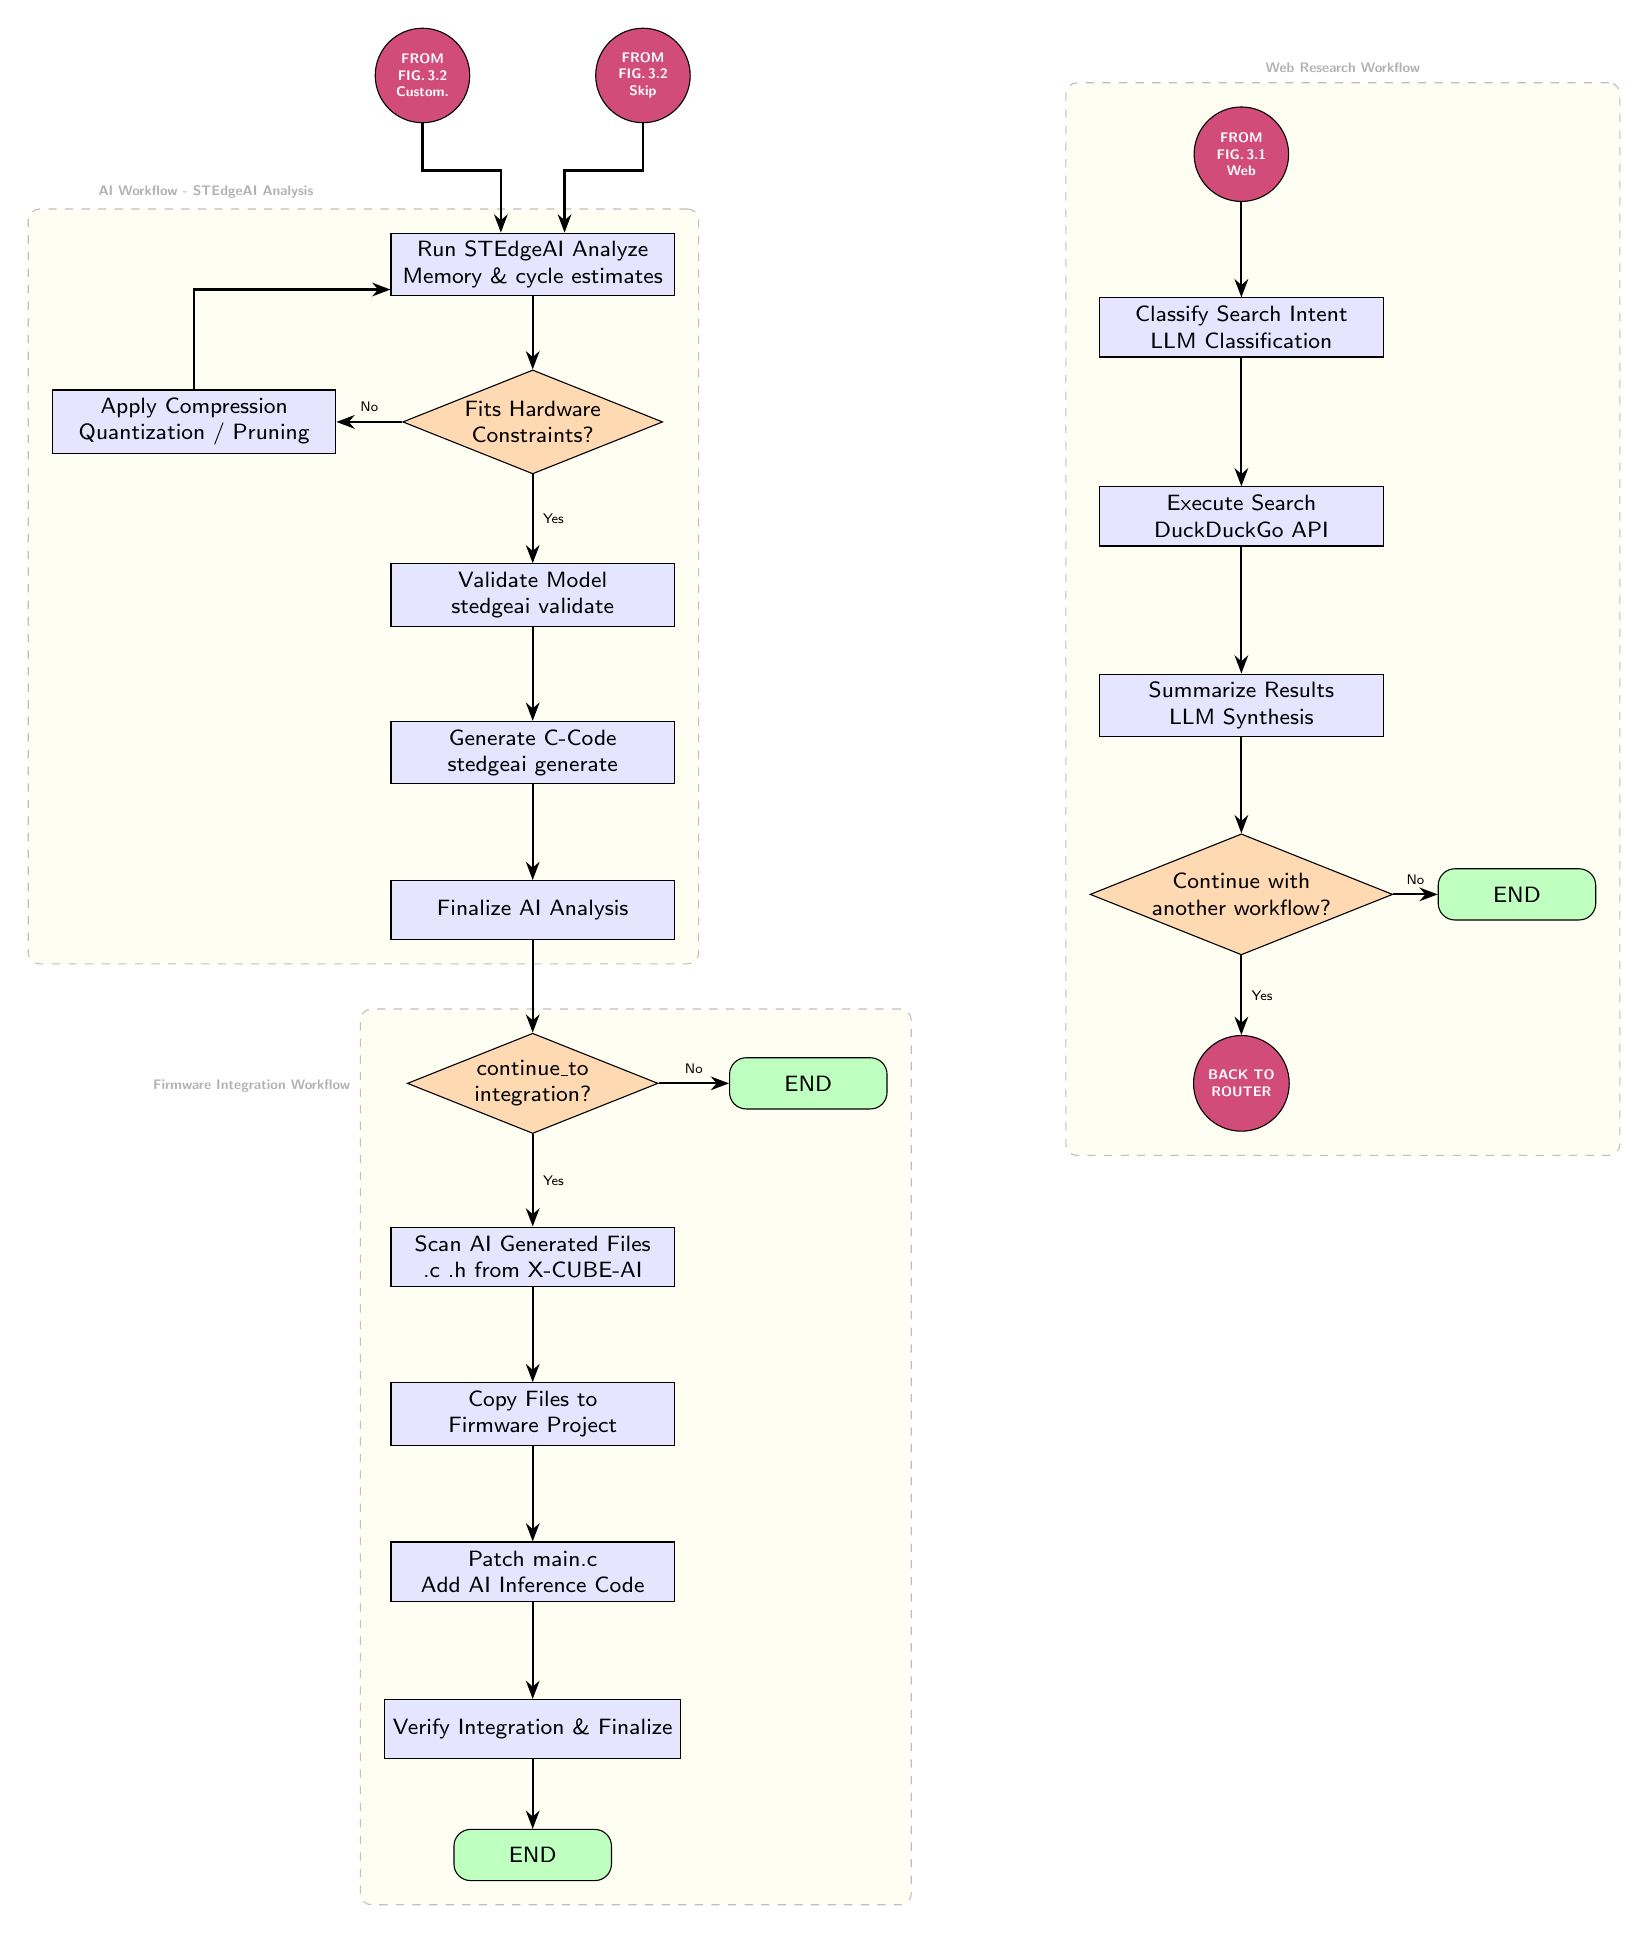
\begin{tikzpicture}[
  every node/.style={font=\sffamily\footnotesize},
  proc/.style={draw, fill=blue!10, rectangle, minimum width=3.6cm,
               minimum height=0.75cm, align=center, inner sep=3pt},
  dec/.style={draw, fill=orange!30, diamond, aspect=2.5,
              align=center, inner sep=1pt, minimum width=3cm, minimum height=1cm},
  se/.style={draw, rectangle, rounded corners=6pt, fill=green!25,
             minimum width=2cm, minimum height=0.65cm, align=center},
  co/.style={draw, circle, fill=purple!70, text=white, minimum size=1.2cm,
             align=center, font=\sffamily\tiny\bfseries},
  wb/.style={draw=gray!50, dashed, rounded corners=4pt, fill=yellow!5, inner sep=0.3cm},
  ar/.style={->, thick, >=Stealth}]

%% --- FROM connectors ---
\node[co]   (F3A)  at (-2.9,  0)   {FROM \\ FIG.\,3.2 \\ Custom.};
\node[co]   (F3B)  at (-0.1,  0)   {FROM \\ FIG.\,3.2 \\ Skip};

%% --- STEdgeAI (WF2B) - x shifted -1.5 ---
\node[proc] (ANA)  at (-1.5, -2.4)  {Run STEdgeAI Analyze \\ Memory \& cycle estimates};
\node[dec]  (FIT)  at (-1.5, -4.4)  {Fits Hardware \\ Constraints?};
\node[proc] (CMP)  at (-5.8, -4.4)  {Apply Compression \\ Quantization / Pruning};
\node[proc] (VAL)  at (-1.5, -6.6)  {Validate Model \\ stedgeai validate};
\node[proc] (GEN)  at (-1.5, -8.6)  {Generate C-Code \\ stedgeai generate};
\node[proc] (FIN)  at (-1.5,-10.6)  {Finalize AI Analysis};

%% --- Integration (WF3) ---
\node[dec]  (IGC)  at (-1.5,-12.8) {continue\_to \\ integration?};
\node[se]   (ENDC) at ( 2.0,-12.8){END};
\node[proc] (IGA)  at (-1.5,-15.0) {Scan AI Generated Files \\ .c .h from X-CUBE-AI};
\node[proc] (IGB)  at (-1.5,-17.0) {Copy Files to \\ Firmware Project};
\node[proc] (IGC2) at (-1.5,-19.0) {Patch main.c \\ Add AI Inference Code};
\node[proc] (IGD)  at (-1.5,-21.0) {Verify Integration \& Finalize};
\node[se]   (ENDL) at (-1.5,-22.6) {END};

%% --- Web Search (WF4, right column, shifted down) ---
\node[co]   (F3C)  at ( 7.5, -1.0) {FROM \\ FIG.\,3.1 \\ Web};
\node[proc] (WSA)  at ( 7.5, -3.2) {Classify Search Intent \\ LLM Classification};
\node[proc] (WSB)  at ( 7.5, -5.6) {Execute Search \\ DuckDuckGo API};
\node[proc] (WSC)  at ( 7.5, -8.0) {Summarize Results \\ LLM Synthesis};
\node[dec]  (WSCT) at ( 7.5,-10.4) {Continue with \\ another workflow?};
\node[co]   (BCK)  at ( 7.5,-12.8) {BACK TO \\ ROUTER};
\node[se]   (ENDW) at ( 11.0,-10.4) {END};

%% --- Arrows: STEdgeAI ---
\draw[ar] (F3A.south) -- ++(0,-0.6) -| (ANA.135);
\draw[ar] (F3B.south) -- ++(0,-0.6) -| (ANA.45);
\draw[ar] (ANA)  -- (FIT);
\draw[ar] (FIT.west) -- node[above,font=\sffamily\tiny]{No} (CMP.east);
\draw[ar] (CMP.north) |- (ANA.190);
\draw[ar] (FIT.south) -- node[right,font=\sffamily\tiny]{Yes} (VAL.north);
\draw[ar] (VAL) -- (GEN);
\draw[ar] (GEN) -- (FIN);
\draw[ar] (FIN) -- (IGC);

%% --- Arrows: Integration ---
\draw[ar] (IGC.east)  -- node[above,font=\sffamily\tiny]{No}  (ENDC.west);
\draw[ar] (IGC.south) -- node[right,font=\sffamily\tiny]{Yes} (IGA.north);
\draw[ar] (IGA) -- (IGB);
\draw[ar] (IGB) -- (IGC2);
\draw[ar] (IGC2) -- (IGD);
\draw[ar] (IGD) -- (ENDL);

%% --- Arrows: Web Search ---
\draw[ar] (F3C.south)  -- (WSA.north);
\draw[ar] (WSA)  -- (WSB);
\draw[ar] (WSB)  -- (WSC);
\draw[ar] (WSC)  -- (WSCT);
\draw[ar] (WSCT.south) -- node[right,font=\sffamily\tiny]{Yes} (BCK.north);
\draw[ar] (WSCT.east)  -- node[above,font=\sffamily\tiny]{No}  (ENDW.west);

%% --- Bounding boxes ---
\begin{scope}[on background layer]
  \node[wb, fit=(ANA)(FIT)(CMP)(VAL)(GEN)(FIN),
        label={[font=\sffamily\tiny\bfseries,text=gray!60,yshift=+0.1mm,xshift=-20mm]above :AI Workflow - STEdgeAI Analysis}]{};
  \node[wb, fit=(IGC)(ENDC)(IGA)(IGB)(IGC2)(IGD)(ENDL),
        label={[font=\sffamily\tiny\bfseries,text=gray!60, yshift=+10mm]above left:Firmware Integration Workflow}]{};
  \node[wb, fit=(F3C)(WSA)(WSB)(WSC)(WSCT)(BCK)(ENDW),
        label={[font=\sffamily\tiny\bfseries,text=gray!60]above:Web Research Workflow}]{};
\end{scope}
\end{tikzpicture}}
\caption{Detailed Workflow Diagram - STEdgeAI profiling and C-code generation (Workflow~2), firmware integration (Workflow~3), and on-demand web research (Workflow~4).}
\label{fig:detailed_flowchart_part3}
\end{figure}
